%!TEX TS-program = pdflatex
%!BIB program = biber
% -- Author: Jannes Bantje, j.bantje@wwu.de
%!TEX root = bachelor.tex
% -- Author: Jannes Bantje, j.bantje@wwu.de
\documentclass[german,a4paper,draft,index=totoc,toc=listof,fontsize=12,DIV=13,headinclude,twoside,BCOR=12mm,cleardoublepage=empty]{scrreprt}


%-- Basics für graphische Sachen
\usepackage[usenames,x11names]{xcolor} % Die Optionen definieren zusätzliche Farben (siehe Dokumentation)
\usepackage[final]{graphicx}

%-- Figures centering
\makeatletter
\g@addto@macro\@floatboxreset\centering
\makeatother
%Figure barriers
\usepackage{placeins}
\usepackage[labelformat=simple]{subcaption}
\renewcommand\thesubfigure{(\alph{subfigure})}

%-- typografische Verbesserungen, Codierungskram, Schriftwahl und erste Mathepakete
\usepackage{hyphenat}
\usepackage[utf8]{inputenc}
\usepackage[lining,semibold]{libertine}
\usepackage[T1]{fontenc}
\usepackage{textcomp} % verhindert ein paar Fehler bei den Fonts
\usepackage[varl]{zi4}
\usepackage{mathtools,amssymb,amsthm} % Verbesserung von amsmath (die amsmath selbst lädt)
\usepackage[libertine,cmintegrals,bigdelims,varbb]{newtxmath}
\usepackage[ngerman]{babel}
\usepackage[babel=true, tracking=true,final]{microtype}
\usepackage{easybmat}
\usepackage{rotating}

%Tabellen
\usepackage{tabularx}

\usepackage{caption}
\usepackage[Algorithmus]{algorithm} % Wrapper für Pseudo-Code
\usepackage{algpseudocode} % Für Pseudo-Code
\renewcommand{\algorithmiccomment}[1]{{\color{gray}\textit{// #1}}} %Comment-Style
\newenvironment{breakablealgorithm}
{% \begin{breakablealgorithm}
	\begin{center}
		\refstepcounter{algorithm}% New algorithm
		\hrule height.8pt depth0pt \kern2pt% \@fs@pre for \@fs@ruled
		\renewcommand{\caption}[2][\relax]{% Make a new \caption
			{\raggedright\textbf{Algorithmus~\thealgorithm} ##2\par}%
			\ifx\relax##1\relax % #1 is \relax
			\addcontentsline{loa}{algorithm}{\protect\numberline{\thealgorithm}##2}%
			\else % #1 is not \relax
			\addcontentsline{loa}{algorithm}{\protect\numberline{\thealgorithm}##1}%
			\fi
			\kern2pt\hrule\kern2pt
		}
	}{% \end{breakablealgorithm}
	\kern2pt\hrule\relax% \@fs@post for \@fs@ruled
	\end{center}
}

\usepackage{listings}
%\usepackage{fvextra}
%\renewcommand\listoflistingscaption{Liste der Quelldateien}
%\setminted[c++]{
%	linenos,
%	autogobble=true,
%	breaklines=true,
%	numbersep=6pt}
%\setminted[text]{
%	linenos,
%	autogobble=true,
%	breaklines=true,
%	numbersep=6pt}
%
%\newcommand{\java}[1]{\mintinline{java}{#1}}

% \useosf % aktiviert sog. "old style figures", also werden Zahlen – im Text – teilweise unterhalb der Grundlinie angezeigt. Muss man mögen...


%-- Alternative Konfiguration mit XeLaTeX, die ein großes "ß" anzeigen kann!
%-- ACHTUNG: wenn diese benutzt werden soll, dan MUSS man in der ersten Zeile von bachelor.tex "pdflatex" durch "xelatex" ersetzen und natürlich den obigen Block auskommentieren und diesen wiederrum aktivieren!!!

% \usepackage{lmodern}
% \usepackage{mathtools,amssymb,amsthm} % Verbesserung von amsmath (die amsmath selbst lädt)
% \usepackage[libertine,cmintegrals,bigdelims,varbb]{newtxmath}
% \usepackage[no-math]{fontspec}
% \usepackage{polyglossia} % moderner babel-ersatz
% \setmainlanguage[spelling=new,babelshorthands=true]{german}
% \shorthandoff{"}
% \defaultfontfeatures{Mapping=tex-text, Ligatures={Required,Common,Contextual}}
% \setmainfont{LinLibertine}[Extension=.otf,UprightFont=*_R,BoldFont=*_RZ,ItalicFont=*_RI,BoldItalicFont=*_RZI,ItalicFeatures={Ligatures=Historical}]
% \setsansfont{LinBiolinum}[Scale=MatchUppercase, Extension=.otf, UprightFont=*_R, BoldFont=*_RB, ItalicFont=*_RI,BoldItalicFont=*_RBO]
% \setmonofont{Inconsolatazi4}[Scale=MatchUppercase,Extension=.otf,UprightFont=*-Regular,BoldFont=*-Bold,StylisticSet=1]
% \usepackage[final]{microtype}


%-- Zeilenabstand einstellen
\usepackage{setspace}
% Nun kann man, wenn gewünscht den Zeilenabstand zum Beispiel auf 1,5 setzen mit \onehalfspacing

\newcommand{\command}[1]{\texttt{\textbackslash{}#1}}

\newcommand{\pathdiff}[1]{\textbf{#1}}



%-- Mathematikpakete und Einstellungen
\mathtoolsset{centercolon} % sorgt dafür dass := und =: besser aussehen
\usepackage{mathdots} % sorgt dafür, dass Punte wie zB \ddots besser aussehen
\newcommand{\Underbrace}[2]{{\underbrace{#1}_{#2}}} % Underbrace als Befehl in LaTeX-Syntax (und ohne Spacing-Probleme mit nachfolgenden Operatoren...)
\renewcommand{\le}{\leqslant} % ich finde Kleinergleich mit schrägen Strich schöner
\renewcommand{\ge}{\geqslant}

%-- charakteristische-Funktion-/Indikatorfunktion-Eins '\ind'
\usepackage{silence}
\WarningFilter{latexfont}{Size substitutions with differences}
\WarningFilter{latexfont}{Font shape `U/bbold/m/n' in size}
\DeclareSymbolFont{bbold}{U}{bbold}{m}{n}
\DeclareSymbolFontAlphabet{\mathbbold}{bbold}
\newcommand{\ind}{\mathbbold{1}}


\newcommand{\atano}{\text{atan}}
\newcommand{\atant}{\text{atan2}}
%-- Ein sehr hübscher Mengen-Befehl
\newcommand\SetSymbol[1][]{\nonscript\:#1\vert\allowbreak\nonscript\:\mathopen{}}
\providecommand\given{} % to make it exist
\DeclarePairedDelimiterX\set[1]\{\}{\renewcommand\given{\SetSymbol[\delimsize]}#1}

%-- Klammern, Skalarprodukt und Norm
\DeclarePairedDelimiter{\enbrace}{(}{)}
\DeclarePairedDelimiter{\abs}{|}{|}
\DeclarePairedDelimiterX\skal[2]{\langle}{\rangle}{#1\,\delimsize\vert\,#2}
\DeclarePairedDelimiter{\norm}{\lVert}{\rVert}

%-- Differentialrechnung
\newcommand{\mathd}{\mathrm{d}\mkern-0.5mu}
\newcommand{\diff}[2]{\frac{{\partial #1}}{{\partial #2}} }
\newcommand{\diffd}[2]{\frac{\mathd #1}{\mathd #2} }

%-- eigene Befehle
\DeclareMathOperator{\sgn}{sgn}


%-- kommutative Diagramme
\usepackage{tikz-cd} %-- meiner Meinung nach das beste Paket für kommutative Diagramme
\tikzset{% um Kompatibilität mit Babel herzustellen und die angenehme "<label>"-Syntax zu nutzen
  every picture/.append style={
    execute at begin picture={\shorthandoff{"}},
    execute at end picture={\shorthandon{"}}
  }
}
\usetikzlibrary{quotes,babel}
\usepackage{onimage}

%-- Für Literaturangaben, hier wird NICHT das total veraltete bibtex benutzt!
\usepackage[%
	backend=biber,
	sortlocale=auto,
	natbib,
	hyperref,
	backref,
	style=alphabetic % eine unvollständige Auswahl von Styles: ieee, numeric, apa
	]%
{biblatex}
\addbibresource{quellen.bib} % Literaturdatei einlesen

% -- Konfiguration von Hyperref (sorgt für anklickbare Links und ein PDF-Inhaltsverzeichnis)
\usepackage[hidelinks, pdfpagelabels, bookmarksopen=true, bookmarksnumbered=true, linkcolor=black, urlcolor=SkyBlue2, plainpages=false,pagebackref, citecolor=black, hypertexnames=true, pdfborderstyle={/S/U}, linkbordercolor=SkyBlue2, colorlinks=false, backref=false]{hyperref}
\hypersetup{final}

%-- Für Aufzählungen und andere Listen, Anführungszeichen und Zitate
\usepackage[shortlabels]{enumitem} % durch die Option ist die gleiche Syntax wie zB mit dem Paket paralist möglich
\setlist[enumerate,description]{font=\sffamily\bfseries} % sorgt dafür, dass die Labels bei enumerate und description fett sind
\usepackage[german=quotes]{csquotes}

%-- Für hilfreiche Anmerkungen am Seitenrand
\usepackage[obeyDraft,textsize=small]{todonotes}

%-- Kopf- und Fußzeilen bearbeiten
\usepackage{scrpage2}
\pagestyle{scrheadings}
\clearscrheadfoot % Standardkonfiguration löschen
\setheadsepline{1pt}[\color{gray}] % Linie für die Kopfzeile
\automark[section]{chapter} % definiert, welcher Text in den Kolumnentiteln erscheinen soll
\rohead{\rightmark} % section erscheint rechts oben
\lehead{\scshape\leftmark} % chapter erscheint links oben in ist in small caps gesetzt
\ofoot[\pagemark]{\pagemark} % Seitenzahlen immer außen, hier wir auch der plain Stil bearbeitet!
%\ifoot[Titel der Bachelorarbeit]{Titel der Bachelorarbeit}
\renewcommand*{\pnumfont}{\sffamily} % Seitenzahlen in groß und serifenlos
\renewcommand*{\footfont}{\sffamily\color{gray}}
\renewcommand*{\headfont}{\sffamily\color{gray}}



%-- Theorem-Pakete und Konfiguration
\usepackage{thmtools}

\usepackage{bookmark}
% Theoreme als PDF-Lesezeichen
\bookmarksetup{open,numbered}
\makeatletter
\newcommand*{\theorembookmark}{%
  \bookmark[
    dest=\@currentHref,
    rellevel=1,
    keeplevel,
  ]{%
    \thmt@thmname\space\csname the\thmt@envname\endcsname
    \ifx\thmt@shortoptarg\@empty
    \else
      \space(\thmt@shortoptarg)%
    \fi
  }%
}
\makeatother



\declaretheoremstyle[%
	headfont=\sffamily\bfseries,
	notefont=\normalfont\sffamily,
	bodyfont=\normalfont,
	headformat=\NUMBER\ \NAME\NOTE,
	headpunct={},
	postheadspace=\newline,
	postheadhook=\theorembookmark,
	%spaceabove=15pt,
	%spacebelow=10pt,
	mdframed={
		backgroundcolor=gray!20,
		linecolor=gray,
		topline=false,
		bottomline=false,
		rightline=false,
		leftline=false,
		innerbottommargin=6pt,
		innertopmargin=6pt,
	}]%
{mainstyle}
\declaretheoremstyle[%
	headfont=\itshape,
	bodyfont=\normalfont,
	headformat=\NAME \NOTE,
	headpunct=.,
	postheadspace=1ex,
	spacebelow=12pt,spaceabove=2pt,
	qed=\qedsymbol]%
{beweise}

\declaretheorem[name=Definition,parent=section,style=mainstyle]{definition}
\declaretheorem[name=Satz,sharenumber=definition,style=mainstyle]{satz}
\declaretheorem[name=Korollar,sharenumber=definition,style=mainstyle]{korollar}
\declaretheorem[name=Lemma,sharenumber=definition,style=mainstyle]{lemma}
\declaretheorem[name=Proposition,sharenumber=definition,style=mainstyle]{proposition}

\declaretheorem[name=Beweis,numbered=no,style=beweise]{beweis}

\newenvironment{beispiel}{}{\par\medskip}


%Informationen zur Arbeit
\newcommand{\printname}{Lars Haalck}
\newcommand{\printmatrickel}{407 846}
\newcommand{\printtitel}{Entzerrung von Kegeloberflächen aus einer Einkameraansicht basierend auf projektiver Geometrie}
\newcommand{\printort}{Münster}
\newcommand{\printartderarbeit}{Bachelorarbeit}
\newcommand{\printstudiengang}{BSc. Informatik}
\newcommand{\printstudiengrad}{Bachelor of Science}
\newcommand{\printbetreuer}{Dimitri Berh}
\newcommand{\printerstgutachten}{Prof. Dr. Xiaoyi Jiang}
\newcommand{\printzweitgutachten}{Prof. Dr. Klaus Hinrichs}
\newcommand{\printinstitut}{Institut für Informatik}

%\hyphenation{Be"-tween"-ness"--Zen"-tra"-li"-tät}
%\hyphenation{Be-tween-ness Zen-tra-li-tät On-line"=Ver-sand-händ-ler}
\begin{document}
\pagenumbering{Roman} % Seitennummerierung auf römische Zahlen setzen

\listoftodos
\begin{titlepage}
	% ===========
% Titelseite
% ===========

% --- Kopf- und Fusszeilen der Titelseite sind leer
\thispagestyle{empty}

\hspace*{1em}
\vfill
\begin{center}
			\includegraphics[width=10cm]{./images/wwu-logo-neu.pdf}
		\par
		\vspace*{8ex}
\LARGE
			\textsc{\printtitel}
		\par
\normalsize
		\vspace*{8ex}
\large
			\textsc{\printartderarbeit}\\
\normalsize
			zur Erlangung des akademischen Grades\\
\large
			\textsc{\printstudiengrad}
		\par
		\normalsize
		\vspace*{6ex}
			Westfälische Wilhelms-Universität Münster\\
			Fachbereich Mathematik und Informatik\\
			\printinstitut
\end{center}

	\par
	\vspace*{6ex}
Betreuung:\\
	\large
	\textit{\printbetreuer}
	
	\par
	\normalsize
	\vspace*{2ex}
	Erstgutachten:\\
	\large
	\textit{\printerstgutachten}
	
	\par
	\normalsize
	\vspace*{2ex}
	Zweitgutachten:\\
	\large
	\textit{\printzweitgutachten}
	
	\par
	\normalsize
	\vspace*{2ex}
	Eingereicht von:\\
	\large
	\textit{\printname}
	
	\par
	\normalsize
	\vspace*{4ex}
		Münster, \makeatletter
\month@ngerman
\makeatother~\the\year
\vfill
\hspace*{1em}
	
\end{titlepage}

\begin{abstract}
\section*{Zusammenfassung}
\todo{abstract schreiben}
\end{abstract}
\cleardoubleoddemptypage
\tableofcontents
\cleardoubleoddemptypage
\pagenumbering{arabic}
\setcounter{page}{1}
\cleardoubleoddemptypage
%!TEX root = ../bachelor.tex
\chapter{Einleitung}
Drosophilae melanogaster, im Volksmund auch Fruchtfliege genannt, und ihre Larven sind schon seit Jahrzehnten ein wichtiges Untersuchungsobjekt der Biologie. Sie zeichnen sich aus durch einen schnellen Generationswechsel, eine hohe Nachkommenszahl, eine einfache Chromosomenstruktur und können darüber hinaus leicht gehalten und gezüchtet werden.

%\todo{ghosts lass ich weg, weil ich dafür FTIR erklären müsste}
In den vergangenen Jahren wurden verschiedene Versuchsaufbauten zur Untersuchung des Bewegungsmusters von Drosphilae entwickelt.
Als problematisch erwies sich, dass das Verhalten der Larven beim Herausnehmen aus ihren Aufzuchtröhrchen, bedingt durch den ausgesetzten Stress, negativ beeinflusst werden kann.
Es wurde daher ein Aufbau entwickelt, in dem die Larven direkt in ihrem Aufzuchtröhrchen beobachtet werden konnten, wie in Abbildung \ref{fig:oldSetup} schematisch dargestellt.
Die Larven befinden sich hierbei in einem Zylinder, der von insgesamt fünf Kameras beobachtet wird, die jeweils an einen Raspberry Pi angeschlossen sind. Die Kameras nehmen nun simultan ein Bild auf, wobei hier eine Synchronisation notwendig ist. Auf Grund der Krümmung des Zylinders, müssen diese nun entsprechend entzerrt werden. Anschließend werden die fünf entzerrten Bilder zu einem Gesamtbild zusammengefügt.
\begin{figure}[!htb]
	\centering
	\begin{subfigure}{.5\textwidth}
		\centering
		\includegraphics[width=0.95\textwidth]{images/renderCylinder.png}
		\caption{bisheriger Ansatz}
		\label{fig:oldSetup}
	\end{subfigure}%
	\begin{subfigure}{.5\textwidth}
		\centering
		\includegraphics[width=0.95\textwidth]{images/renderCone.png}
		\caption{neuer Ansatz}
		\label{fig:newSetup}
	\end{subfigure}
	\caption{beide Ansätze im Vergleich}
	\label{fig:renderedSetup}
\end{figure}

Um ein bessere4sn Verhältnis zwischen der Anzahl der Kameras und des Aufzuchtgeheges zu erreichen, wäre eine Reduktion der Kameraanzahl wünschenswert.
Statt eines Zylinders wird in einem neuen Aufbau einen Kegel benutzt, wie in Abbildung \ref{fig:newSetup} zu sehen. Das Gehege wird mit einer einzigen Weitwinkelkamera beobachtet. Eine Synchronisation, sowie ein Zusammenfügen von Einzelbilder, ist hier nicht mehr notwendig.
Wie auch bei dem bisherigen Aufbau muss hier jedoch eine Entzerrung durchgeführt werden. Die Larven, die sich am oberen Rand des Kegels befinden scheinen sonst größer, als jene, die sich im unteren Bereich aufhalten. Ein relativer Vergleich der Larven wäre somit nicht möglich.

In dieser Arbeit werden zwei Verfahren zum Entzerren solcher Kegeloberflächen vorgestellt, sodass die relative Vergleichbarkeit der Larven gewährleistet ist.
Dazu wird die Kegeloberfläche mit Hilfe einer geeigneten Abbildung auf die Mantelfläche projiziert.

Im folgenden Kapitel werden zunächst die notwendigen theoretischen Grundlagen erarbeitet.
Anschließend werden beide Verfahren zur Entzerrung von Kegeloberflächen vorgestellt und ihre Funktionsweisen erläutert, woraufhin auf den implementierten Kalibrierungsassistenten eingegangen wird, der diesen Prozess vereinfachen soll.
Im Anschluss werden beide Verfahren gegenüber gestellt und verschiedene Einflussfaktoren in Bezug auf die Präzision und Qualität der Entzerrung untersucht.
Im letzten Kapitel wird ein Fazit gezogen und ein Ausblick auf mögliche Verbesserungsmaßnahmen für die verwendeten Verfahren gegeben.
\todo{evtl vergleichen die beiden Verfahren?}

\cleardoubleoddemptypage
%!TEX root = bachelor.tex
\chapter{Theoretische Grundlagen}
theorie
\cleardoubleoddemptypage
%!TEX root = bachelor.tex
\chapter{Methodik}
\label{ch:method}

In diesem Kapitel stellen wir ein Verfahren vor, dass ermöglicht anhand eines Bildes (siehe Einleitung).

Zunächst gehen wir auf das verwendete Kalibrierungsmuster ein, woraufhin die genaue Vorgehensweise zur Entfaltung erläutert wird. 

Die geometrischen Eigenschaften des Kegelstumpfs $(r, R, \Delta H)$ können gemessen und somit als bekannt angenommen werden. 
Darüber hinaus nehmen wir an, dass sich das Zentrum des kleineren Kreises im links-händigen Weltkoordinatensystem an der Positon $(0,0,0)$ (siehe Abbildung \ref{fig:coneFrustum}) befindet. Durch diese Einschränkung gehen jegliche absolute Größenverhältnisse verloren. Die Larven können jedoch weiterhin relativ zu einander verglichen werden. 


\section{Kalibrierungsmuster}
\label{s:calibrationPattern}
Um eine Beziehung zwischen Bildpunkten und Kegelpunkten herstellen zu können, ist ein Kalibrierungsmuster notwendig.

Die Wahl des Kalibrierungsmusters spielt dabei eine entscheidende Rolle bei der Robustheit und Präzision der Entfaltung. Es muss gewährleistet sein, dass die charakteristischen Merkmale des Musters, auch bei leichten Abweichungen der Kamera vom Lot und schlechteren Beleuchtungssituationen zuverlässig erkannt werden. Das Muster muss darüber hinaus so entworfen sein, dass beim Zusammenlegen im Kegel, dessen geometrische Eigenschaften nicht verfälscht, sondern realitätsgetreu wiedergeben werden. 

Wir haben uns für ein Muster entscheiden, dass in äquidistanten Abständen $\Delta R$, beginnend mit dem kleinen Radius $r$ des Kegelstumpfs (siehe Abbildung \ref{fig:coneFrustum}) Kreislinien und in gleichen Winkelabständen $\Delta \alpha$ auf der Seitenhöhe Liniensegmente besitzt. Das zusammengelegte Muster ist in Abbildung \ref{fig:calibrationPatternTop} zu sehen, beziehungsweise das entfaltete in \ref{fig:calibrationPattern}. Die Anzahl der Kreislinien wird mit $n$ gekennzeichnet, die Anzahl sichtbarer Liniensegmente im Kegel mit $m$. Zu beachten ist, dass bedingt durch das Entfalten, in \ref{fig:calibrationPattern}  ein Liniensegment doppelt zu sehen ist. Die schwarzen Kreise bezeichnen wir als Samples. 

Dadurch dass die Geometrie des Kegels bekannt ist, kann jedem Sample nun ein Punkt auf dem Kegel im Weltkoordinatensystem zugeordnet werden. Da ein Kegel beliebig um die $Y$ Achse rotiert werden, kann ist diese Abbildung zunächst nicht eindeutig. Dazu nehmen wir an, dass das Liniensegment mit dem kleinsten Winkel zur $X$-Achse mit dem Kegelwinkel $\theta = 0$ korrespondiert (siehe \ref{eq:paramFrustum}).

\begin{figure}[!htb]
	\centering
	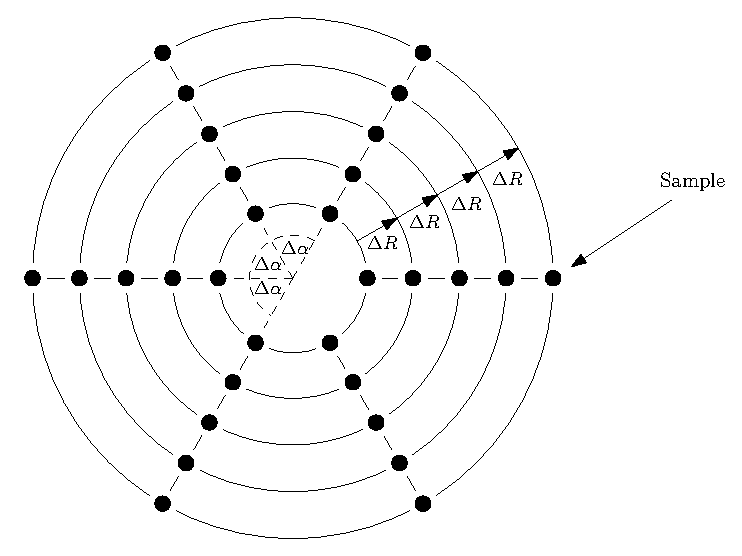
\includegraphics[scale=.8]{images/calibrationPatternTop.eps}
	\caption{Kalibrierungsmuster von oben mit $n = 5, m = 6$}
	\label{fig:calibrationPatternTop}
\end{figure}


\begin{figure}[!htb]
	\centering
	\includegraphics[scale=.7]{images/calibrationPattern2.eps}
	\caption{Kalibrierungsmuster entfaltet mit $n = 5, m = 6$}
	\label{fig:calibrationPattern}
\end{figure}


\subsection{Anzahl der Samples}
Die Anzahl der Samples sollte groß genug sein, um möglichst viel geometrische Informationen des Kegels zu erhalten, aber klein genug, dass eine Detektion der Samples problemlos möglich ist. Insbesondere auf dem innersten Kreis, macht sich eine zu hohe Sampleanzahl negativ bemerkbar, da der Abstand zueinander sehr klein wird, was eine Detektion erschwert. Des Weiteren sollte noch ein möglichst großer Teil der Kreislinien zu sehen bleiben, da diese für die Ellipsendetektion benötigt werden. 


\todo{warum gerade dieses muster? warum ist das so gut? wie berechnet man das muster? welche eigenschaften hat es?}


Bilder von kegel mit muster drin?

\section{Intrinsische Kamerakalibrierung}
\todo{hier mit linsenverzerrungen}
Bedingt durch die Wahl einer Weitwinkelkamera, enthält die Linse der Kamera eine starke tonnenförmige (nach außen gewölbte) Verzerrung. Ohne eine intrinsische Kamerakalibrierung würde. Es werden nur die intrinsischen Parameter benötigt.


\begin{figure}[!htb]
	\centering
\begin{subfigure}{.5\textwidth}
	\centering
	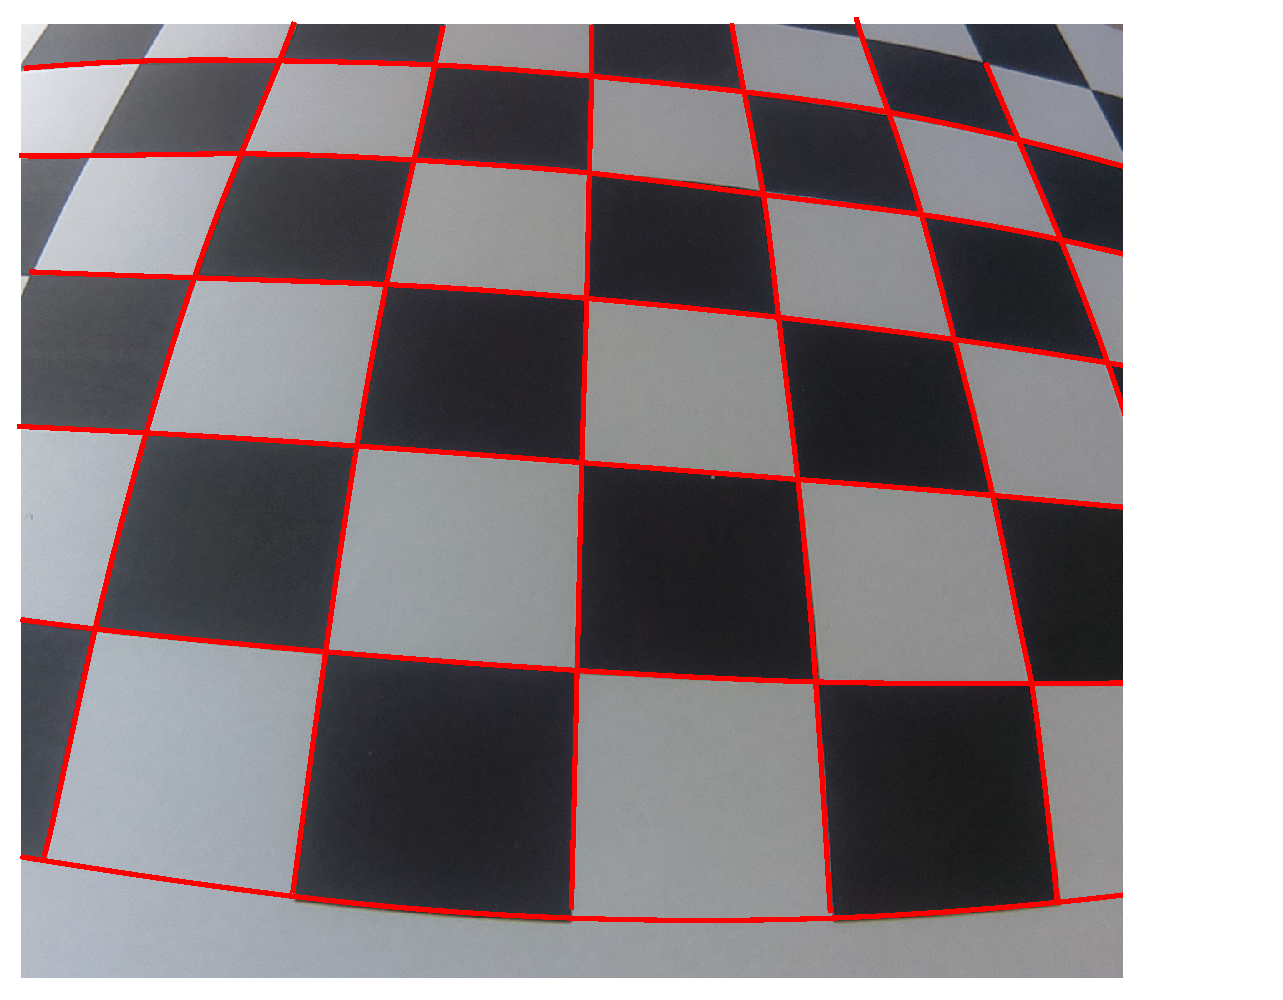
\includegraphics[scale=.35]{images/calibrationRaspi.eps}
	\caption{vor Kalibrierung}
	\label{fig:calibDist}
\end{subfigure}%
\begin{subfigure}{.5\textwidth}
	\centering
	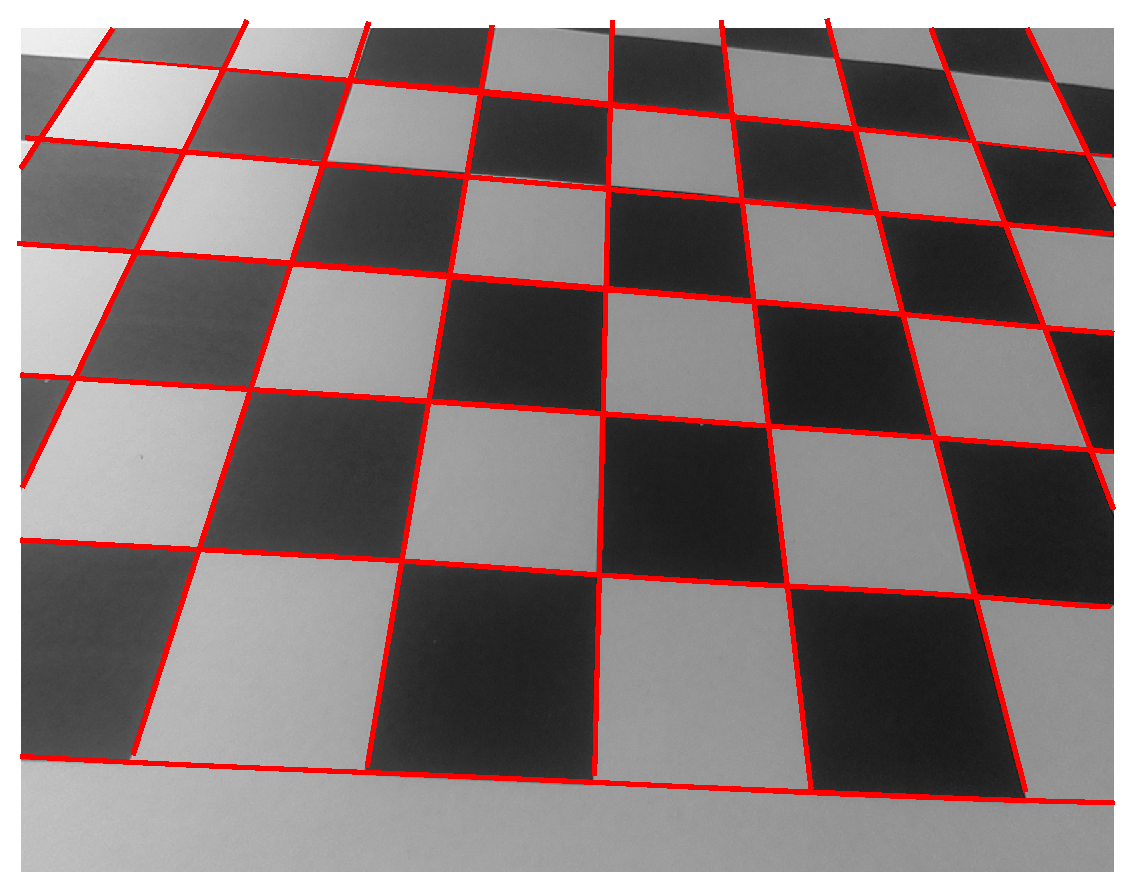
\includegraphics[scale=.4]{images/calibrationRaspi2.eps}
	\caption{nach Kalibrierung und Entzerrung}
	\label{fig:calibUndist}
\end{subfigure}
\caption{Kamerakalibrierung}
\label{fig:calib}
\end{figure}


\section{Detektion der charakteristischen Punkte}

Nach der Kamerakalibrierung und entsprechender Entzerrung werden die Bildkoordinaten der Samples bestimmt. Dazu wird ein Blob-Detektor (siehe Kapitel \ref{s:blob}) benutzt. 
Um ein Sample korrekt detektieren zu können, muss sich der Punkt farblich stark von seiner Umgebung abheben (siehe Definition: Blob \ref{def:blob}). Insbesondere dürfen die Kreislinien und Liniensegmente des Kalibrierungsmusters also nicht durchgezogen sein. Nach der Detektion werden die Blobs nach folgenden Kriterien gefiltert:

\begin{itemize}
	\item \textbf{Fläche:} zu kleine Blobs werden verworfen
	\item \textbf{Rundheit:} zu unrude Blobs werden verworfen. Rundheit ist hier definiert als $circ = \frac{4\pi\cdot \textrm{Fläche}}{\left(\textrm{Umfang}\right)^2}\in[0,1]$, wobei ein Kreis mit $circ = 1$ maximal rund ist. 
	\item  \textbf{Konvexität:} zu unkonvexe Blobs werden verworfen. Konvextität ist hier definiert als $conv = \frac{\textrm{Fläche Blob}}{\textrm{Fläche konvexe Hülle}}$
\end{itemize}

In Abbildung \ref{fig:blobDetect} ist beispielhaft links ein Grauwertbild und rechts die detektierten Blobs auf dem gleichen Bild nach der Kameraentzerrung zu sehen.


\begin{figure}[!htb]
	\centering
	\begin{subfigure}{.5\textwidth}
		\centering
		\includegraphics[width=.9\textwidth]{images/coneRasp.jpg}
		\caption{Grauwertbild}
	\end{subfigure}%
	\begin{subfigure}{.5\textwidth}
		\centering
		\includegraphics[width=.9\textwidth]{images/coneRaspDetectedDots.png}
		\caption{detektierte Blobs in grün}
	\end{subfigure}
	\caption{Detektion der Samples}
	\label{fig:blobDetect}
\end{figure}


\section{Ellipsen-Detektion}
\label{s:ellipseDetection}
Nachdem die Sample-Positionen bestimmt wurden, muss für jeden Sample entschieden werden, auf welcher der Kreislinien er liegt. Da die Kreise, bedingt durch perspektivische Verzerrung, zu  Ellipsen werden, wird eine Verfahren 
benötigt, dass Ellipsen erkennt. 

Zunächst werden die Kanten mit Hilfe von Canny (\ref{s:canny}) detektiert (siehe Abbildung \ref{fig:canny}). 

\begin{figure}[!htb]
	\centering
	\begin{subfigure}{.5\textwidth}
		\centering
		\includegraphics[width=.9\textwidth]{images/grey.png}
		\caption{Grauwertbild}
		\label{fig:beforeCanny}
	\end{subfigure}%
	\begin{subfigure}{.5\textwidth}
		\centering
		\includegraphics[width=.9\textwidth]{images/canny.png}
		\caption{Canny-Kanten}
		\label{fig:afterCanny}
	\end{subfigure}
	\caption{Canny-Kantendetektion auf Grauwertbild}
	\label{fig:canny}
\end{figure}

Anschließend versuchen wir möglichst genau das Zentrum der innersten Ellipsen zu bestimmen.
Wir benutzen dafür Hough-Transformationen, um Linien im Canny-Bild zu detektieren.
Es werden anschließend die Schnittpunkte aller Liniensegmente bestimmt. Bedingt durch Ungenauigkeiten beim Ausschneiden und Zusammenlegen im Kegel und perspektivischer Verzerrung, schneiden sich nicht alle Liniensegmente in einem Punkt.
Darüber hinaus werden, auf Grund der Liniendicke auf dem Kalibrierungsmuster, durch Canny viele Linien doppelt erkannt\footnote{Dies ist kein Widerspruch zur Eindeutigkeit von Canny-Kanten (siehe \ref{s:canny}), da dickere Linien zwei Kanten besitzen. Stellt man sich ein relativ breites Liniensegment vor, so gibt es einmal den Übergang vom Hintergrund auf die Linie, sowie den Übergang von der Linie wieder auf den Hintergrund}. Auch ein inhomogener Hintergrund, erschwert die Schnittpunktsbestimmung. Um also möglichst robust einen Kandidaten auszuwählen, wird zuerst der Median der $x$-Koordinaten der Schnittpunkte und dann der Median der $y$-Koordinaten bestimmt. Die erhaltenen Koordinaten bilden den Schnittpunkt (siehe Abbildung \ref{fig:houghLines}).

\begin{figure}[!htb]
	\centering
	\includegraphics[scale=.25]{images/houghLines.png}
	\caption{Hough-Transformation zur Linien-Detektion (in rot gekennzeichnet) und bestimmter Schnittpunkt (in grün) }
	\label{fig:houghLines}
\end{figure}

Von diesem Schnittpunkt aus werden, in einer vorher definierte Anzahl, gleichmäßig, in alle Richtungen Strahlen ausgesendet.
Trifft ein Strahl ein weißes Pixel, wird dessen Position gekennzeichnet, trifft er den Rand des Bildes, wird er ignoriert. In Abbildung \ref{fig:rayCastWOE} sind die getroffenen weißen Pixel und der zugehörige Aussendepunkt eingezeichnet. 

\begin{figure}[!htb]
	\centering
	\begin{subfigure}{.5\textwidth}
		\centering
		\includegraphics[width=.9\textwidth]{images/rayCast0.png}
		\caption{bestimme Pixel-Positionen}
		\label{fig:rayCastWOE}
	\end{subfigure}%
	\begin{subfigure}{.5\textwidth}
		\centering
		\includegraphics[width=.9\textwidth]{images/rayCast0Ellipse.png}
		\caption{bestimme Ellipse (grün)}
		\label{fig:rayCastWE}
	\end{subfigure}
	\caption{Ellipsendetektion: bestimme Pixel-Positionen (weiß), Aussendepunkt (gelb)}
	\label{fig:rayCast}
\end{figure}

Mit Hilfe der Postionen der weißen Pixel, wird anschließend durch RANSAC (siehe Kapitel \ref{s:ransac}) eine Ellipse geschätzt. 

Es wird konkret für sechs zufällig ausgewählte Punkte das lineare Gleichungssystem:
\[
\begin{pmatrix}
x_1^2 & y_1^2 & x_1y_1 & x_1 & y_1 & 1\\
\vdots &\vdots & \vdots & \vdots &\vdots & \vdots\\
\vdots &\vdots & \vdots & \vdots &\vdots & \vdots\\
x_6^2 & y_6^2 & x_6y_6 & x_6 & y_6 & 1
\end{pmatrix} \begin{pmatrix}
a \\ b \\ c \\ d \\ e \\ f
\end{pmatrix} = \begin{pmatrix}
0 \\ 0 \\ 0 \\ 0 \\ 0 \\ 0
\end{pmatrix}
\]

gelöst, was auf der Gleichung \ref{eq:ellipseQuadratic} aus Kapitel \ref{s:ellipse} basiert. Nach dem Lösen wird geprüft ob, es sich tatsächlich um eine Ellipse handelt und mittels Hauptachsentransformation (siehe Kapitel \ref{s:ellipse}) in die Ellipsenform $(x_0,y_0,a,b,\phi)$ umgewandelt. 


Um die, für RANSAC benötigte, Distanz zu berechnen, wird das Verfahren aus Kapitel \ref{sc:distPointEllipse} genutzt, was die exakte euklidische Distanz eines Punktes zu einer Ellipse bestimmt. Ein Verfahren wie das Verfahren der kleinsten Quadraten funktioniert hier nicht, da die weißen Pixel bezüglich einer zu bestimmenden Ellipse, ausreißerbehaftet sind. Wird zum Beispiel auf Grund schlechter Lichtverhältnisse eine Kreislinie nicht deutlich aufgenommen, kann es in dem Kantenbild (Abbildung \ref{fig:canny}) zu "`Löchern"' in den Kreislinien kommen und folglich treffen die ausgesendeten Strahlen die nächst äußere Kreislinie (siehe Abbildung \ref{fig:rayCastR}). Da die Laufzeit nicht im Vordergrund steht, kann eine großzügige Schätzung des Fehleranteils von $\epsilon = 0.4$ mit einer gewünschten Wahrscheinlichkeit $p = 0.9999$ gewählt werden, was zu einer Mindestanzahl an Iterationen von circa $200$ führt (siehe Kapitel \ref{s:ransac}). Die letztendlich bestimmten Ellipsen sind beispielhaft in Abbildung \ref{fig:detectedEllipses} zu sehen.  


\begin{figure}[!htb]
	\centering
	\begin{subfigure}{.5\textwidth}
		\centering
		\includegraphics[scale=.6]{images/rayCastRobust.png}
		\caption{bestimme Pixel-Positionen}
		\label{fig:rayCastRWOE}
	\end{subfigure}%
	\begin{subfigure}{.5\textwidth}
		\centering
		\includegraphics[scale=.6]{images/rayCastRobustEllipse.png}
		\caption{bestimme Ellipse (grün)}
		\label{fig:rayCastRWE}
	\end{subfigure}
	\caption{Ellipsendetektion bei Ausreißern}
	\label{fig:rayCastR}
\end{figure}


\begin{figure}[!htb]
	\centering
	\includegraphics[scale=.25]{images/detectedEllipses.png}
	\caption{detektierte Ellipsen}
	\label{fig:detectedEllipses}
\end{figure}

\newpage
\section{Zuordnung der Punkte}
\label{s:pointMapping}
Nach der Bestimmung der Ellipsen muss jede Sample-Positionen der zugehörigen Kreislinie, sowie Liniensegment zugeordnet werden, um seine Position auf dem Kegel bestimmen zu können. 
Zunächst wird für jeden Punkt diejenige Kreislinie ausgewählt, dessen zugehörige Ellipse die kürzeste Distanz zu ihm hat (siehe Abbildung \ref{fig:ellipseMapping}).

Mit Hilfe dieser Zuordnung können die Ellipsen aus Kapitel \ref{s:ellipseDetection} erneut geschätzt werden. Diesmal wird das Verfahren der kleinsten Quadrate genutzt, da nur die ausreißerfreihen Samples als Messdaten dienen und wir eine optimale Lösung für alle Samples anstreben.  

Um nun die Samples auch ihren Liniensegmenten zuzuordnen, wird zunächst der Mittelpunkt der Samples auf der innersten Ellipse bestimmt. Anschließend werden die Samples auf der innersten Ellipsen nach dem Winkel der Verbindungslinien zwischen Sample und Mittelpunkt mit der $X$-Achse sortiert. 
Die restlichen Samples können nicht nach dem gleichen Schema sortiert werden, da der bestimme Mittelpunkt nicht der genaue Schnittpunkt aller Liniensegmente ist. Der Winkel zwischen der Samples auf einem Liniensegment und des bestimmen Mittelpunkts ist also nicht identisch. 
Stattdessen wird für jedes Sample  auf den darauffolgenden Ellipsen, das Sample auf der vorherigen Ellipse mit der kürzesten Distanz bestimmt. 

Die Samples können nun entsprechend sortiert werden. Die zugeordneten Liniensegmente sind exemplarisch in Abbildung \ref{fig:lineMapping} zu sehen. 


\begin{figure}[!htb]
	\centering
	\begin{subfigure}{.5\textwidth}
		\centering
		\includegraphics[width=.9\textwidth]{images/ellipseMapping.png}
		\caption{Zuordnung von Punkten zu Ellipsen}
		\label{fig:ellipseMapping}
	\end{subfigure}%
	\begin{subfigure}{.5\textwidth}
		\centering
		\includegraphics[width=.9\textwidth]{images/lineMapping.png}
		\caption{Zuordnung von Punkten zu Liniensegmenten}
		\label{fig:lineMapping}
	\end{subfigure}
	\caption{Zuordnung von Punkten zu Ellipsen (links) und Liniensegmenten (rechts)}
	\label{fig:mapping}
\end{figure}


\section{Weltkoordinaten bestimmen}

Aus dem vorherigen Kapitel wissen wir nun für jedes Sample den Ort auf dem Kegel. Wir können die 3D-Koordinaten also folgendermaßen angeben:

Ohne Beschränkung der Allgemeinheit, seien die Ellipsen $i = 0,\dotsc,n - 1$ aufsteigend nach ihrer "`Größe"'\footnote{Etwas formaler, könnte man die Ellipsen hier nach ihrem Flächeninhalt sortieren. Für Ellipsen $E_0(x_0,y_0,a_0, b_0, \theta_0)$ und $E_1(x_1,y_1,a_1, b_1,\theta_1)$ gilt $E_0 \leq E_1$ g.d.w. $\pi\cdot a_0 \cdot b_0 \leq \pi \cdot a_1 \cdot b_1$} sortiert, so wie es das Verfahren in \ref{s:ellipseDetection} beschreibt.
Außerdem seien die Liniensegmente $j = 0,\dotsc,m - 1$ aufsteigend nach Winkel mit der $X$-Achse, wie in \ref{s:pointMapping} beschrieben, sortiert. 
Eine Sample kann also eindeutig durch ein Tupel $(i,j) \in [0,n-1]\times [0,m-1]$ identifiziert werden und $(x_{ij},y_{ij},z_{ij})$ bezeichne seine Koordinaten im Weltkoordinatensystem. 

Analog zur parametrischen Darstellung von Kegelstümpfen (Gleichung \ref{eq:paramFrustum}) in Kapitel \ref{s:cone} ergibt sich:

\begin{equation*}
\begin{aligned}
x_{ij} &= r_i~cos \theta_j \\
y_{ij} &= h_i\\
z_{ij} &= r_i~sin \theta_j
\end{aligned}
\end{equation*}
$\forall (i,j) \in [0,n-1]\times [0,m-1]$ mit 
\begin{equation*}
\begin{aligned}
r_i &= r + \frac{i}{n}\cdot(R - r) \quad&\forall i\in[0,n-1]\\
h_i &= \frac{i}{n}\cdot\Delta H &\forall i\in[0,n-1]\\
\theta_j &= \frac{j}{m-1} \cdot  2\pi  &\forall j\in[0,m-1]
\end{aligned}
\end{equation*}

\section{Entfaltung}
Die eigentliche Entfaltung des Kegels kann mit zwei unterschiedlichen Ansätzen realisiert werden. 
Die erste Möglichkeit ist die \textit{Vorwärtsentfaltung}. Hierbei wird für jedes Pixel auf dem Kegelbild eine 3D-Koordinate durch geeignete Interpolation bestimmt und dann auf die Mantelfläche abgebildet. Beim zweiten Ansatz, der \textit{Rückwärtsentfaltung}, wird ein Punkt von der Mantelfläche zurück auf den Kegel abgebildet und von dort mit einer Projektionsmatrix auf die Bildebene projiziert und dann interpoliert. 

Im folgenden wird genauer auf beide Verfahren eingegangen, sowie deren Probleme erläutert. \todo{hier schon erläutern oder erst in späteren kapiteln?}

\subsection{Vorwärtsentfaltung}
Bei der \textit{Vorwärtsentfaltung} muss wie oben erwähnt zu jedem Pixel die zugehörige 3D Koordinate im Weltkoordinatensystem berechnet werden. Da bisher jedoch nur die Positionen der Samples bekannt sind muss hier 

Zunächst betrachten wir diejenigen Pixel, die sich weder auf einer Kreislinie, noch auf einem Liniensegment befinden. Es gibt zu einem Pixel $P$ also immer vier Sample-Nachbarn $(bl, br, tr, tl)$. Diese Situation ist in Abbildung \ref{fig:radialInterpolation} illustriert. 

Nachdem die vier Nachbarn bestimmt wurden, können im ersten Schritt die Abstände $d_1$ und $d_2$ zu inneren Ellipse $E_b$, respektive äußeren Ellipse $E_t$ berechnet werden. Mithilfe dieser Abständen kann nun eine \textit{Interpolationsellipse}~$E_1$ definiert werden als
\begin{equation*}
	E_{int} = \left(\frac{d_1}{d_1 + d_2}\right) \cdot E_t + \left(\frac{d_2}{d_1 + d_2}\right) E_b,
\end{equation*}

wobei eine Multiplikation mit einem Skalar alle Charakteristika einer Ellipse skaliert. Der Drehwinkel $\theta$ wird hierbei bei $2\pi$ umgebrochen. Eine Addition geschieht elementweise. Im nächsten Schritt wird der Schnittpunkt $L$ mit dem Liniensegment $\overline{bltl}$, sowie der Schnittpunkt $R$ mit dem Liniensegment $\overline{brtr}$ bestimmt. 

Da sich $tl$, $L$ und $bl$ nun auf einem gemeinsamen Liniensegment befinden, kann bezüglich der Weltkoordinaten linear interpoliert werden. Analoges gilt für $tr$,$R$ und $br$. 

Die drei Punkte $(L, P, R)$ befinden sich auf der Interpolationsellipse und somit können die  Winkel $(\phi_L, \phi_P, \phi_R)$ bezüglich des gemeinsamen Ellipsenkoordinatensystems bestimmt werden. 

Analog zu oben werden die 3D-Koordinaten von $P$ als lineare Interpolation zwischen den gerade bestimmen 3D-Koordinaten von $L$ und $R$ bestimmt. Als Interpolationsfaktor benutzen wir
$\frac{\phi_L - \phi_P}{\phi_L - \phi_R}$


\begin{figure}[!htb]
	\centering
	\includegraphics[scale=.6]{images/radialInterpolation.eps}
	\caption{Interpolation}
	\label{fig:radialInterpolation}
\end{figure}


\begin{figure}[!htb]
	\centering
	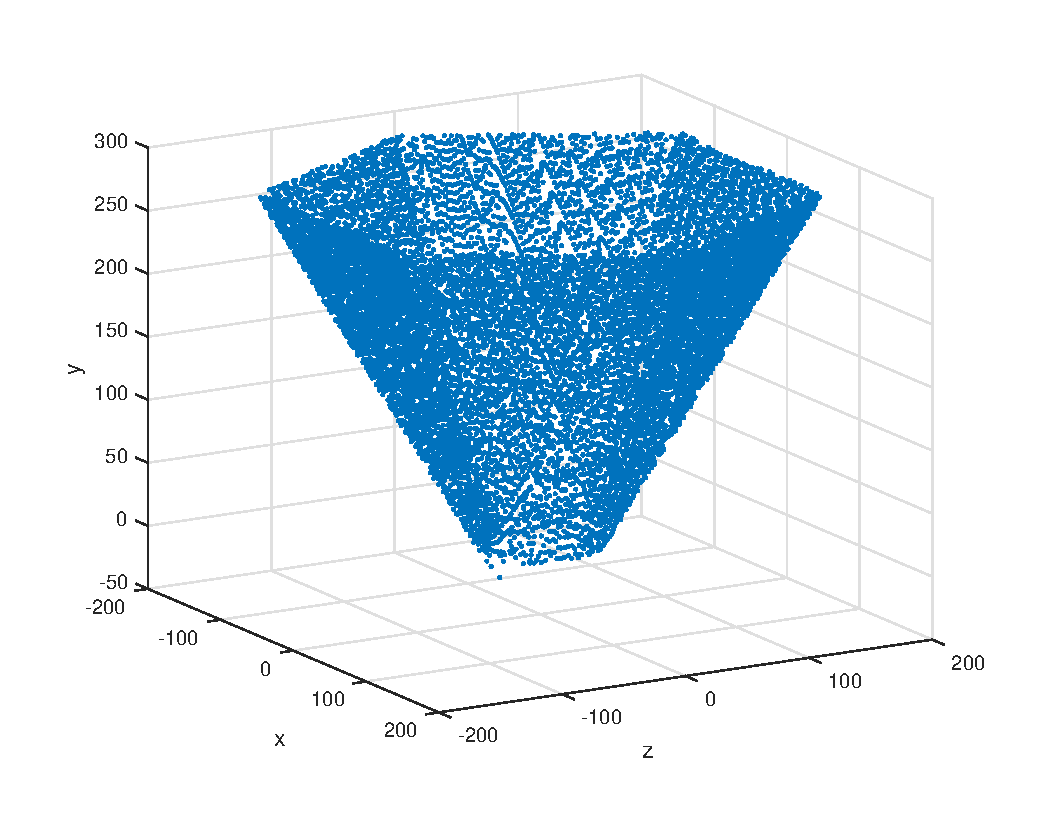
\includegraphics[scale=.7]{images/3d_interpol.eps}
	\caption{Interpolation}
	\label{fig:3DInterpol}
\end{figure}

Analog werden die auf Liniensegmenten befindlichen Punkte einfach linear interpoliert. Die Punkte, die sich auf Kreislinien befinden werden über Winkel interpoliert. 

Jedes Pixel hat nun 3D-Koordinaten im Kegel erhalten, die beispielhaft in Abbildung \ref{fig:3DInterpol} zu sehen sind. \todo{gehören Probleme schon hier her? oder erst bei analyse?}
Anhand der Abbildung lässt sich das erste Problem bei der Vorwärtsentfaltung feststellen. Zwischen den Samples auf einer Kreislinie sollten die interpolierte Positionen nach außen gewölbt sein, da ein Kegel rund ist. Da wir jedoch Interpolieren und nicht Extrapolieren, gehen die Werte nie über die zur Interpolation genutzten Werte hinaus. Konkreter kann eine interpolierte Position keine größeren oder kleineren $X$ und $Z$ Koordinaten erhalten, als die der genutzten Samples. Diese wäre jedoch notwendig, sodass die Rundung des Kegels erhalten bleibt. Die Oberfläche des Kegels scheint eckig. 

Neben der außerdem sehr hohen Laufzeit, bedingt durch die komplexe Interpolation, ergibt sich noch ein weiteres Problem, dass sich erst bei der Entfaltung ergibt. 

Die eigentliche Entfaltung geschieht über die Abbildung \ref{eq:coneToLateral}, die in Kapitel \ref{s:cone} konstruiert wurde. Die erhaltenen Werte müssen anschließend skaliert werden, da im entfalteten Bild sonst 1 mm einem Pixel entspreche. Es ergibt sich das entfaltete Bild, wie in Abbildung \ref{fig:forwardUnfold} dargestellt. Auch schon bei kleinen Skalierungen entstehen auffällige "`Löcher"' im entfalteten Bild. Grund dafür ist, dass jedes Pixel aus dem Ursprungsbild auf eine 2D-Koordinate der Mantelfläche abgebildet wird. Auch nach einer Skalierung handelt es sich bei diesen Werten im Allgemeinen nicht um ganzzahlige Werte. Es muss im entfalteten Bild gerundet werden. Auch wenn Rundungsfehler nicht entständen, fehlte es einfach an genügend Informationen, gerade in den inneren, kleineren Regionen des Ursprungsbild.

Da wir von dem Ursprungsbild aus auf das entfaltete Bild abbilden, ist außerdem eine Interpolation auf dem Ursprungsbild nicht möglich, da wir vorher nicht genau wissen, wo Löcher entstehen. Man müsste als entweder auf dem resultierendem Bild interpolieren (siehe Kapitel \ref{ch:summary}), oder zu gegebenen Löchern über die Umkehrabbildung auf dem Ursprungsbild interpolieren. 

\begin{figure}[!htb]
	\centering
	\begin{subfigure}{.5\textwidth}
		\centering
		\includegraphics[width=.9\textwidth]{images/coneRasp.jpg}
		\caption{Ursprungsbild}
	\end{subfigure}%
	\begin{subfigure}{.5\textwidth}
		\centering
		\includegraphics[angle=-90, width=.9\textwidth]{images/coneRaspUnWarpForward.png}
		\caption{entfaltetes Bild}
	\end{subfigure}
	\caption{Vorwärtsentfaltung}
	\label{fig:forwardUnfold}
\end{figure}

Es bietet sich dann jedoch an, direkt die Umkehrabbildung zu nutzen, was die Motivation hinter der Rückwärtsentfaltung ist.

\subsection{Rückwärtsentfaltung}
Bei der Rückwärtsentfaltung gehen wir von dem entfalteten Bild aus und bestimmen zunächst mit der Umkehrabbildung \ref{eq:LateralToCone} aus Kapitel \ref{s:cone}, die 3D Kegelkoordinaten. Mit Hilfe einer Projektionsmatrix werden diese 3D-Koordinten dann auf Bildkoordinaten abgebildet.

Konkret lösen wir das überbestimmte lineare Gleichungssystem \ref{eq:DLT} aus Kapitel \ref{ch:theory} mittels \textit{Direct Linear Transformation}.
Die resultierenden Bildkoordinaten sind im Allgemeinen nicht ganzzahlig. Es kann hier allerdings im Gegensatz zur Vorwärtsentfaltung einfach auf dem Ursprungsbild interpoliert werden. 


\begin{figure}[!htb]
	\centering
	\begin{subfigure}{.5\textwidth}
		\centering
		\includegraphics[width=.9\textwidth]{images/coneRasp.jpg}
		\caption{Ursprungsbild}
	\end{subfigure}%
	\begin{subfigure}{.5\textwidth}
		\centering
		\includegraphics[angle=-90, width=.9\textwidth]{images/coneRaspUnWarpReverse.png}
		\caption{entfaltetes Bild}
	\end{subfigure}
	\caption{Rückwärtsentfaltung}
	\label{fig:reverseUnfold}
\end{figure}

\cleardoubleoddemptypage
%!TEX root = bachelor.tex
\chapter{Implementierung}
\label{ch:implementation}

Zwecks Vereinfachung des Kalibrierungsprozesses wurde ein Assistent in Form einer graphischen Benutzerschnittstelle programmiert. 

Im ersten Schritt des Assistenten wird dabei optional eine intrinsische Kamerakalibrierung durchgeführt (siehe Abbildung \ref{fig:wizard1}). 
\begin{figure}[!htb]
	\centering
	\includegraphics[width=0.9\textwidth]{images/GUI/calibWizard1_1.PNG}
	\caption{Kalibrierungsassistent: intrinsische Kamerakalibrierung}
	\label{fig:wizard1}
\end{figure}

Anschließend wird die eigentliche Kegelkalibrierung ausgeführt. Dabei wird zunächst das Kalibrierungsbild geladen und gegebenenfalls nach einer stattgefundenen intrinsischen Kalibrierung entzerrt. Es werden nun die Sample-Positionen detektiert und der Nutzer hat die Möglichkeit zu überprüfen, ob alle Positionen korrekt detektiert wurden und andernfalls fehlerhafte Punkte zu entfernen und / oder Punkte hinzuzufügen. Im Anschluss werden die Ellipsen und Liniensegmente bestimmt und Punktkorrespondenzen hergestellt (siehe Abbildung \ref{fig:wizard2}).

\begin{figure}[!htb]
	\centering
	\includegraphics[width=0.9\textwidth]{images/GUI/calibWizard2_1.PNG}
	\caption{Kalibrierungsassistent: Kegelkalibrierung}
	\label{fig:wizard2}
\end{figure}

Im letzten Schritt kann zwischen beiden Entfaltungsverfahren gewählt werden. Anschließend können die Einstellungen in eine XML-Datei exportiert werden, in der, neben der Kamera-Matrix und Verzerrungskoeffizienten, auch die zwei Abbildungsmatrizen des ausgewählten Verfahrens gespeichert werden. 


Die Abbildungsmatrizen sind dabei wie folgt aufgebaut. Als $dst$ bezeichnen wir das entfaltete Bild. $src$ ist das Ursprungsbild.

Bei der Vowärtsentfaltung gilt:
\[
dst(map_x(x,y), map_y(x,y)) = src(x,y),
\]

wobei $map_x$ und $map_y$ die Abbildungsmatrizen sind und die gleiche Größe wie das Ursprungsbild haben. Da wird bei der Entfaltung die Größe des Ergebnisbildes benötigen, und wir diese bei der Erstellung der Abbildungsmatrizen berechnet haben, sind Breite und Höhe, in $map_x(0,0)$, respektive $map_y(0,0)$, kodiert. Wir verlieren damit die Information $dst(0,0)$ im Ergebnisbild. Dieses Pixel ist aber ohnehin null (siehe zum Beispiel Abbildung \ref{fig:forwardUnfold} in Kapitel \ref{s:unfolding}). 

Bei der Rückwärtsentfaltung gilt:
\[
dst(x,y) = src((map_x(x,y),map_y(x,y)),
\]
wobei $map_x$ und $map_y$ wieder die Abbildungsmatrizen sind und hier die  gleiche Größe wie das entfaltete Bild haben. Eine Kodierung wie bei der Vowärtsentfaltung ist hier also nicht notwendig.

\cleardoubleoddemptypage
%!TEX root = bachelor.tex
\chapter{Analyse}
\label{ch:analysis}
In diesem Kapitel bla bla bla.


\section{Vergleich Vorwärtsentfaltung und Rückwärtsentfaltung}
In Kapitel \ref{ch:method} haben wir festgestellt, dass das entfaltete Bild mittels Vorwärtsentfaltung Löcher enthält. Es ist hierbei von Interesse wie sich die Anzahl der Löcher bei einer Änderung der Auflösung verhält. Der Einfluss der Ausgabeauflösung auf die Anzahl der Löcher lässt sich in Abbildung \ref{fig:influenceRes} ablesen. 

\begin{figure}[!htb]
	\centering
	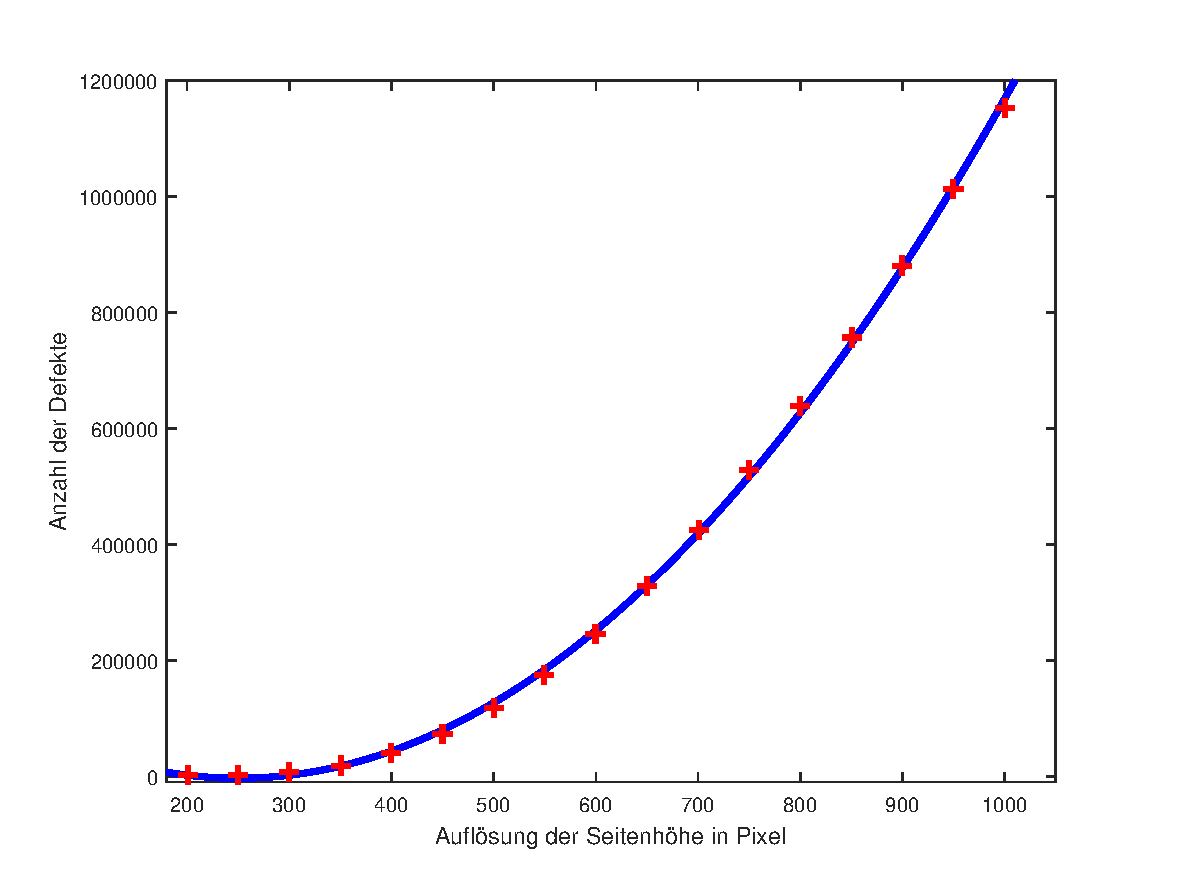
\includegraphics[width=\textwidth]{images/numberOfHoles.eps}
	\caption{Einfluss der Ausgabeauflösung auf die Anzahl der Löcher}
	\label{fig:influenceRes}
\end{figure}

Wie erwartet verhält sich die Anzahl der Löcher quadratisch zur gewählten Ausgabeaufösung. Der Informationsgehalt (Pixelanzahl) des Ursprungsbild bleibt natürlich trotz erhöhter Ausgabeauflösung konstant. Da sich die Auflösung der Seitenhöhe quadratisch zur Gesamtanzahl der Pixel verhält, ist auch ein quadratisches Wachstum der Anzahl der Löcher zu erwarten. 
\bigskip

Als Reprojection-Fehler einer Abbildung wird die Distanz zwischen einem gemessenem Punkt und einem korrespondierendem projizierten Punkt bezeichnet. 

Im Falle der Rückwärtsentfaltung sind die gemessenen Punkte die Bildpositionen der Samples im Ursprungsbild. Da die Geometrie des Kegels bekannt ist, wissen wir wo die Samples auf dem entfalteten Bild sein müssen (siehe Parametrisierung der Mantelfläche \ref{eq:paramLateral} in Kapitel \ref{ch:theory}). Wir können nun diese Positionen mit Hilfe der Abbildung zur Entfaltung und der Projektionsmatrix zurück auf das Ursprungsbild abbilden. Diese Punkte sind die projizierten Punkte. Da die Abbildung von der Mantelfläche zur Kegeloberfläche exakt ist, ist der Reprojection-Fehler der Rückwärtsentfaltung alleine durch die Projektionsmatrix definiert. 

Bei der Vorwärtsentfaltung sind die gemessenen Punkte gegeben durch die bekannten Sample-Positionen auf der Mantelfläche. Die Projizierten erhält man, nach der Abbildung der detektierten Sample-Positionen des Ursprungsbild auf die Mantelfläche. Der Reprojection-Fehler ist also alleine durch die Genaugkeit der Sample-Detektion definiert und somit bei diesem Verfahren immer nahe null. 

Obwohl das Endergebnis, bedingt durch die Löcher, bei der Vorwärtsentfaltung optisch schlechter ist, ist der Reprojection-Fehler also bei der Vorwärtsentfaltung immer kleiner. 
Als Vergleich zwischen den beiden Verfahren eignet sich der Reprojection-Fehler also nicht.

Wir entscheiden uns rein optisch und auf Grund der schlechteren Laufzeit bei der Vorwärtsentfaltung für die Rückwärtsentfaltung. 
Alle weiteren Auswertungen beziehen sich von nun an auf die Rückwärtsentfaltung.

\section{Einfluss der intrinsischen Kalibrierung}
Ein wichtiger Einflussfaktor auf die Qualität der Entfaltung ist die intrinsische Kamerakalibrierung, die vor der eigentlichen Kegelkalibrierung stattfindet. Ihre Hauptaufgabe besteht darin, die Linsenverzerrungen der Kamera zu kompensieren. 

Wir messen den Einfluss der Kamerakalibrierung mit Hilfe des Reprojection-Fehlers. Dazu betrachten wir fünf verschiedene Bilder, die ein Mal mit und ein Mal ohne intrinsische Kalibrierung entfaltet werden. Bei beiden Gruppen wird anschließend jeweils der Reprojection-Fehler bestimmt und verglichen. Die Ergebnisse sind in \ref{fig:influenceCalib} zu sehen. In der linken Abbildung sind hierbei die Fehler im kalibrierten Fall zu erkennen, im Linken die Unkalibrierten. In der Abbildung ist dabei ein Kreuz bei $(u,v)$, falls die Abweichung des projizierten Punktes in $x$-Richtung $u$, sowie in $y$-Richtung $v$ beträgt. 

\begin{figure}[!htb]
	\centering
	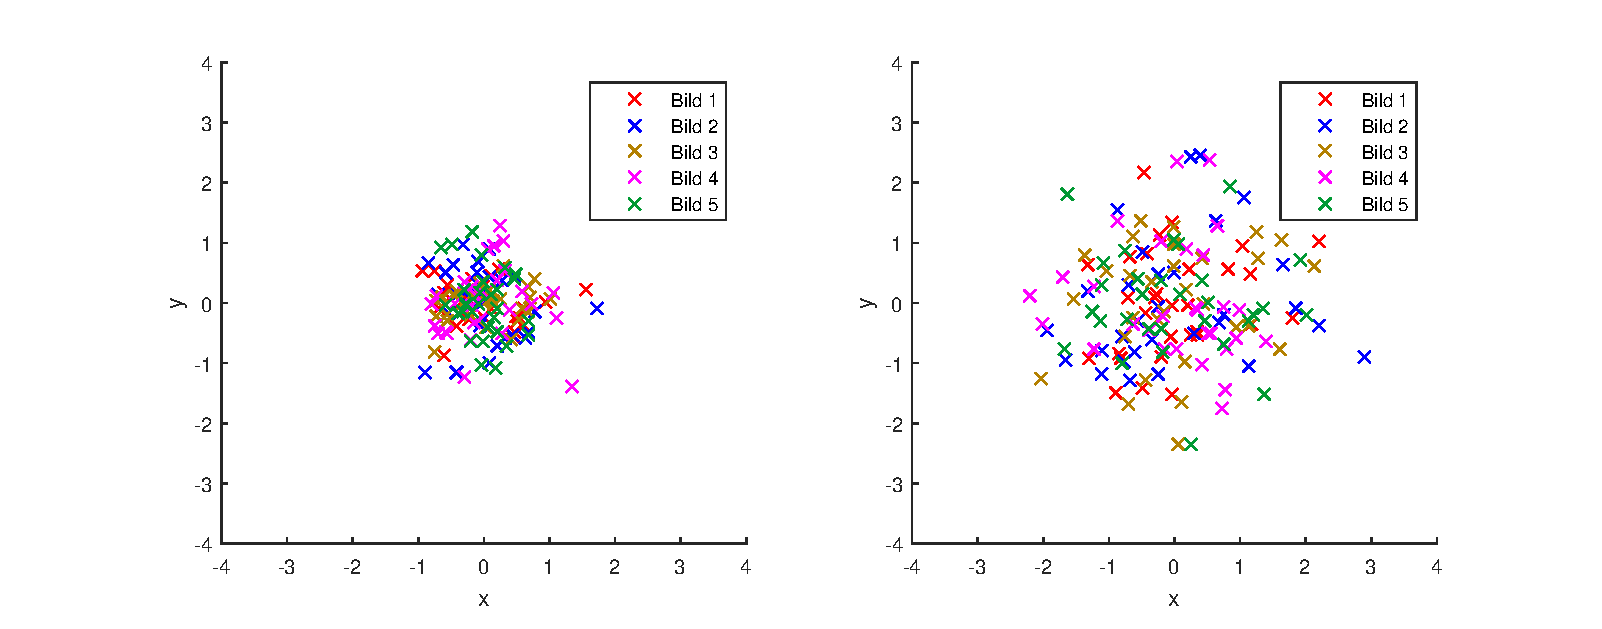
\includegraphics[width=\textwidth]{images/reprojectionErrorReverse.eps}
	\caption{Einfluss der intrinsischen Kalibrierung}
	\label{fig:influenceCalib}
\end{figure}


Es ist klar zu erkennen, dass die Reprojection-Fehler bei den Bildern ohne intrinsische Kamerakalibrierung wesentlich größer ist. Der starke Einfluss kommt unter Anderem daher, dass wir ein Weitwinkelkamera mit starker Tonnenverzerrungen eingesetzt haben. Ohne eine Modellierung der Linsenverzerrungen weichen die Abstände zwischen den Sample-Positionen stark von der Realität ab. Die Projektionsmatrix wird mit fehlerhaften Daten bestimmt. 

\section{Einfluss der Rotation der Kamera}
Um den Einfluss der Rotation der Kamera zu untersuchen, wurde der Kegel mit Kalibrierungsmuster in Blender gerendert, da die Kameraposition dann genau bekannt ist und äußere Faktoren wie Lichtverhältnisse und inhomogene Hintergründe kontrolliert werden können. 

\begin{figure}[!htb]
	\centering
	\begin{subfigure}{.5\textwidth}
		\centering
		\includegraphics[width=.9\textwidth]{images/blender0.png}
		\caption{bei 0°}
	\end{subfigure}%
	\begin{subfigure}{.5\textwidth}
		\centering
		\includegraphics[width=.9\textwidth]{images/blender12.png}
		\caption{bei 12°}
	\end{subfigure}
	\label{fig:blender}
	\caption{gerendeter Kegel mit Kalibrierungsmuster in Blender}
\end{figure}


Es werden anschließend Bilder erzeugt, in denen in 1° Schritten die Kamera von 0° bis 12° um die $X$-Achse rotiert wird. Für jedes dieser Bilder wird anschließend eine Rückwärtsentfaltung durchgeführt und der durchschnittliche Reprojection-Fehler bestimmt. Abbildung \ref{fig:influenceRot} zeigt, dass der Reprojection-Fehler relativ rotationsinvariant ist. 


\begin{figure}[!htb]
	\centering
	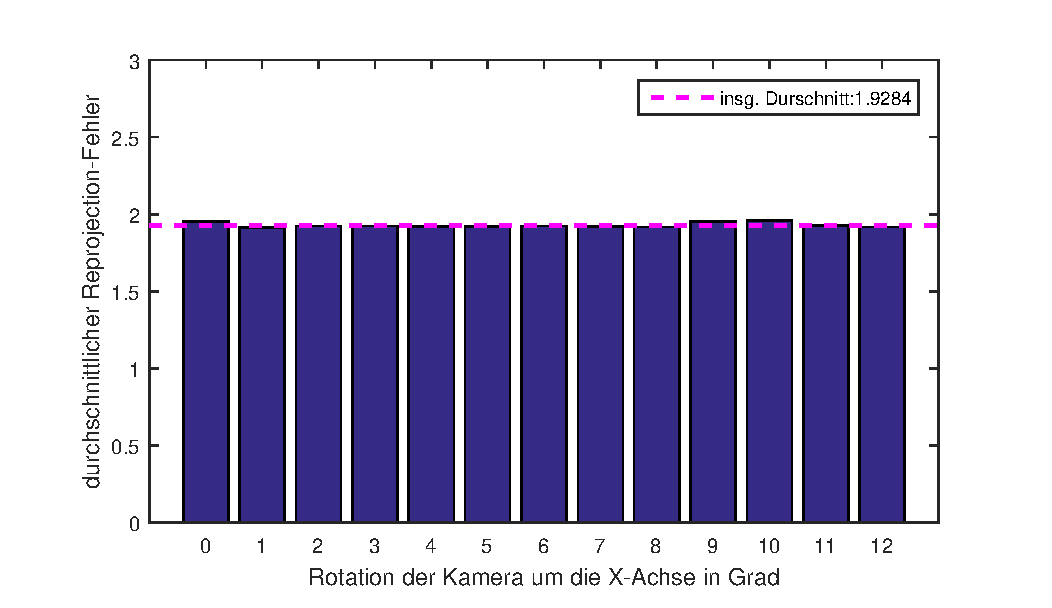
\includegraphics[width=\textwidth]{images/reprojectionErrorDeg2.eps}
	\caption{Einfluss der Rotation der Kamera}
	\label{fig:influenceRot}
\end{figure}


\section{Laufzeit der Entfaltung}


Raspberry Pi 2 Model B:
\begin{itemize}
	\item 900MHz ARM Cortex-A7 CPU
	\item 1GB RAM
	\item GCC-4.9.2
	\item Opencv 2.4.13
\end{itemize}

\begin{figure}[!htb]
	\centering
	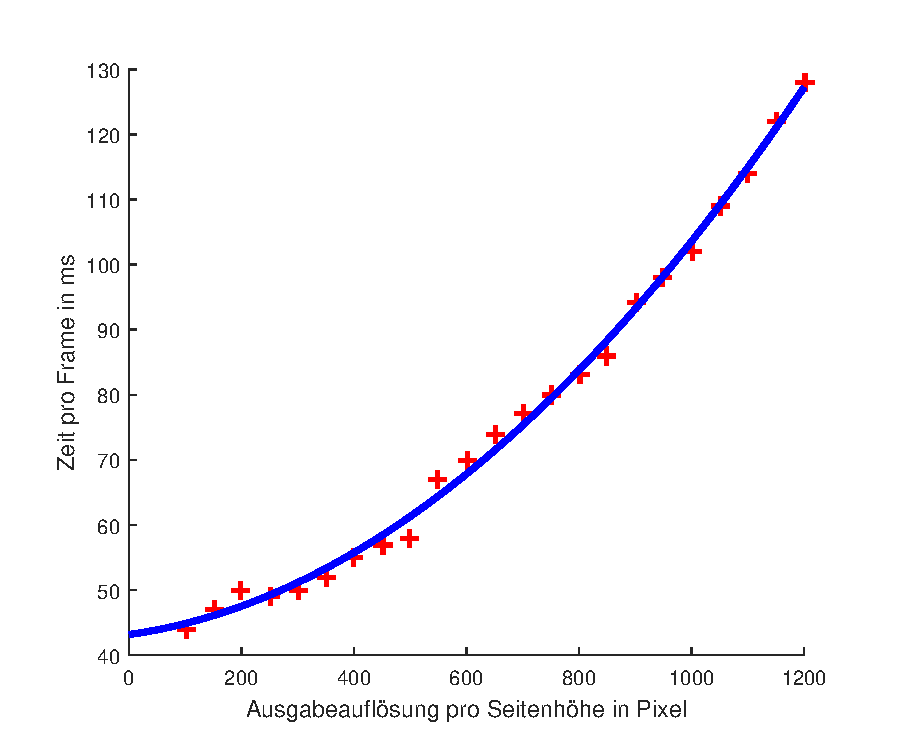
\includegraphics[width=\textwidth]{images/runningTimePerSlantheight.eps}
	\caption{Einfluss der Ausgabeauflösung auf die Laufzeit}
	\label{fig:influenceRes2}
\end{figure}




\bigskip\bigskip

projektionsfehler bei dem einen
anzahl löcher bei dem anderen



robustheit reverse warping? bestimmung der keypoints?







\section{Evaluierung des RANSAC zur Ellipsendetektion}
Die robuste Ellipsendetektion ist ein wichtiger Schritt bei der Entfaltung. Bei beiden Verfahren werden die bestimmten Ellipsen genutzt um Korrespondenzen zwischen den Sample-Positionen und Punkten auf dem Kegel im Weltkoordinatensystem herzustellen. Bei der Vorwärtsentfaltung werden die Ellipsen darüber hinaus benötigt, um für die restlichen Pixel geeignet 3D-Koordinaten interpolieren zu können. Es ist also von großem Interesse wie gut die Ellipsendetektion mittels RANSAC funktioniert.  


\begin{figure}[!htb]
	\centering
	\begin{subfigure}{.5\textwidth}
		\centering
		\includegraphics[width=.9\textwidth]{images/ransac50_0.png}
		\caption{gestörte Messdaten}
	\end{subfigure}%
	\begin{subfigure}{.5\textwidth}
		\centering
		\includegraphics[width=.9\textwidth]{images/ransac50_1.png}
		\caption{detekt. Ellipsen: RANSAC (grün), LSQ (cyan)}
	\end{subfigure}
	\label{fig:bla}
	\caption{Vergleich RANSAC und LSQ bei gleichverteilten Ausreißern $\epsilon = 0.5, p = 0.99$}
\end{figure}

\begin{figure}[!htb]
	\begin{subfigure}{.5\textwidth}
		\centering
		\includegraphics[width=.9\textwidth]{images/ransacShadow25_0.png}
	\end{subfigure}%
	\begin{subfigure}{.5\textwidth}
		\centering
		\includegraphics[width=.9\textwidth]{images/ransacShadow25_1.png}
	\end{subfigure}
	\begin{subfigure}{.5\textwidth}
		\centering
		\vspace{0.2cm}
		\includegraphics[width=.9\textwidth]{images/ransacShadow40_0.png}
	\end{subfigure}%
	\begin{subfigure}{.5\textwidth}
		\centering
		\vspace{0.2cm}
		\includegraphics[width=.9\textwidth]{images/ransacShadow40_1.png}
	\end{subfigure}
	\caption{Vergleich RANSAC und LSQ bei Schattenellipsen mit $p = 0.99$ und $\epsilon = 0.25$ (oben), $\epsilon = 0.4$ unten, links gestörte Messdaten, rechts detektierte Ellipsen RANSAC (grün), LSQ (cyan)}
	\label{fig:blubb}
\end{figure}
























\cleardoubleoddemptypage
%!TEX root = ../bachelor.tex
\chapter{Fazit und Ausblick}
Parallelisierung?
geht immer, weil Imageprocessing.

hough evtl besser probalistic oder richtungasinformationen mit nehmen



iteratives verfahren zum minimieren des reprojection fehlers ausprobieren
robustes projektionsgedöns

Um die Löcher bei der Vörwärtsentfalung zu schließen, könnte man eine Delaunay-Triangulation durchführen. 
Da das Verfahren jedoch ohne Triangulation schon relativ rechenintensiv ist, und die Rückwärtsentfaltung sehr gute Ergebnisse liefert wurde dieses Möglichkeit nicht weiter untersucht.
\begin{figure}[!htb]
	\centering
	\begin{subfigure}{.9\textwidth}
		\centering
		\includegraphics[angle=-90, width=.8\textwidth]{images/delaunay1.png}
		\caption{Triangulation mit $10\%$ der Punkte}
	\end{subfigure}
	\begin{subfigure}{.9\textwidth}
		\centering
		\includegraphics[angle=-90, width=.8\textwidth]{images/delaunay2.png}
		\caption{Triangulation mit $40\%$ der Punkte}
	\end{subfigure}
	\label{fig:delaunay}
	\caption{Delaunay-Triangulation}
\end{figure}

\begin{equation}
	G(x,y) = \frac{((x - x_0)\cos\theta + (y - y_0)\sin\theta)^2}{a^2} + \frac{((x - x_0)\sin\theta - (y - y_0)\cos\theta)^2}{b^2} - 1 = 0
\end{equation}

\begin{equation}
	E = E_M + E_A + E_S
\end{equation}

\begin{equation}
\begin{aligned}
E_M &= -\alpha\frac{1}{n}\sum_{i=0}^{n-1}I_M(p_i) \\
E_A &= \beta\frac{1}{n}\sum_{i=0}^{n-1}\left(I_O(pi) - \atant{\left(\frac{\partial G}{\partial y}(p_i), \frac{\partial G}{\partial x}(p_i)\right)}\right)^2 \\
E_S &= \gamma\frac{1}{n}\sum_{i=0}^{n-2}\abs{p_i - p_{i+1}}
\end{aligned}
\end{equation}

Man macht die Initialellipse möglichst größ und bestimmt dann numerisch, beispielsweise durch Gradient Descent, ein Minimum der Funktion. Der Term $E_M$ wird minimal, wenn entlang der Ellipse die Kantenstärke (\textit{\textbf{M}agnitude}) groß ist. Der Term $E_A$ wird minimal wenn die Winkel der Normalenvektoren ähnlich zu denen der Kanten sind (\textit{\textbf{A}ngle}) und $E_S$ wird minimal, wenn die Distanz aufeinanderfolgender Ellipsepunkte klein wird, also die Ellipse als ganzes klein wird (\textit{\textbf{S}ize}). Der Term lässt die Ellipse also schrumpfen. $\alpha, \beta$ und $\gamma$ steuern hierbei den Einluss der einzelnen Terme. Das Problem bei diesem Ansatz, ist dass die Funktion auch nach starker Gaussglättung, schnell in kleine lokale Minima läuft, obwohl ein wesentlicher stärkeres Minimum in näherer Umgebung wäre. Darüber hinaus muss für ein robustes Optimierungsverfahren der Gradient und im Besten Fall sogar die Hesse-Matrix zur Verfügung gestellt werden. 



\todo{Literatur checken, ins besondere seitenangaben}
\cleardoubleoddemptypage
\appendix % hier beginnt der Anhang
\listoffigures
\cleardoubleoddemptypage
\listoftables
%\cleardoubleoddemptypage
%\listof{algorithm}{Algorithmenverzeichnis}
%\cleardoubleoddemptypage
%\listoflistings
\cleardoubleoddemptypage
\printbibliography
\cleardoubleoddemptypage
\input{chapter/eidesstattliche.tex}

\nocite{*}
\end{document}
